% !TEX root = ../report.tex
\chapter{Evaluation}
In this chapter it will be described how the proposed approaches were compared against the standard implementation and how they were evaluated.\\
At first the data sets used for the comparison and the evaluation are described, then the \acf{ROS} setup will be explained and in the last section, the evaluation procedure itself will be described.

\section{Data sets}
Both of the used data sets were captured in a room equipped with a motion tracking system, VICON, which provided the ground truth for the comparison and the evaluation. As the whole setup is based on \ac{ROS}, the data sets were recorded with rosbags. The rosbags contain at least the following topics:
\begin{itemize}
  \item The grayscale images as sensor\_msgs.msg.Image in the topic /cam0/image\_raw
  \item The ground truth as geometry\_msgs.msg.PointStamped in the topic /camera\_imu/vrpn\_client/estimated\_transform respective
\end{itemize}

The recorded rosbags were afterwards splitted into parts which do not contain any loop closure as loop closures would prohibit a fair comparison between the standard and the proposed new map merging approach.

For the evaluation each client took the data from a seperate splitted rosbag simulating two clients running the same time in the same area.

\subsection{Hand held}
The hand held data set (vi\_loops\_close and vi\_loosp\_far) was recorded with a camera rig walking loops while facing the wall. In the data set ``vi\_loops\_close'', a frame of it shown in \autoref{fig:dataset_close}, the camera was close to the wall. In the data set ``vi\_loops\_far'', a frame of it shown in \autoref{fig:dataset_far}, the camera was far from the wall.

\begin{figure}[H]
  \centering
  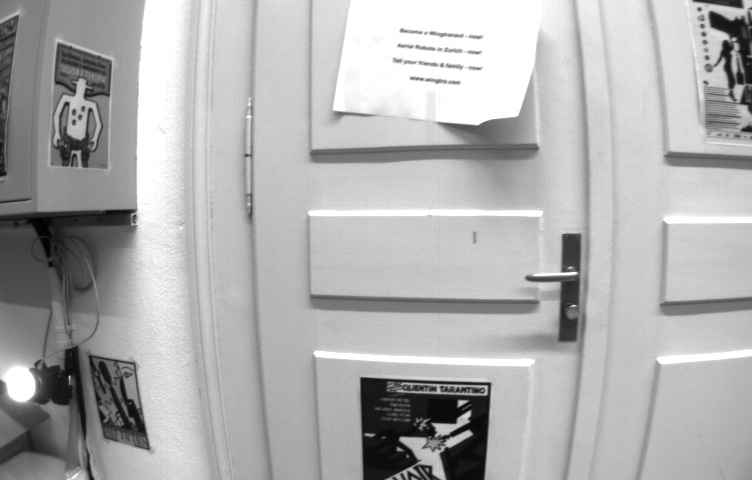
\includegraphics[width=0.75\textwidth]{images/frame0000}
  \caption{Frame from the hand held data set close to the wall}
  \label{fig:dataset_close}
\end{figure}

\begin{figure}[H]
  \centering
  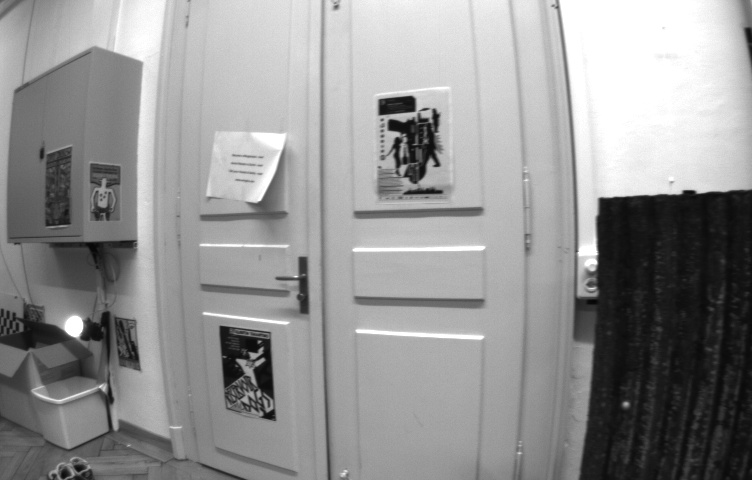
\includegraphics[width=0.75\textwidth]{images/frame0014}
  \caption{Frame from the hand held data set far from the wall}
  \label{fig:dataset_far}
\end{figure}

\subsection{\acf{UAV}}
The \ac{UAV} used to record this data set (vi\_loops\_uav) is shown in \autoref{fig:uav}. In this data set loops were flown while the camera of the \ac{UAV} was facing the wall. A frame of the recorded data set is shown in \autoref{fig:dataset_uav}.

\begin{figure}[H]
  \centering
  \includegraphics[width=0.75\textwidth]{images/uav}
  \caption{The used \ac{UAV}}
  \label{fig:uav}
\end{figure}

\begin{figure}[H]
  \centering
  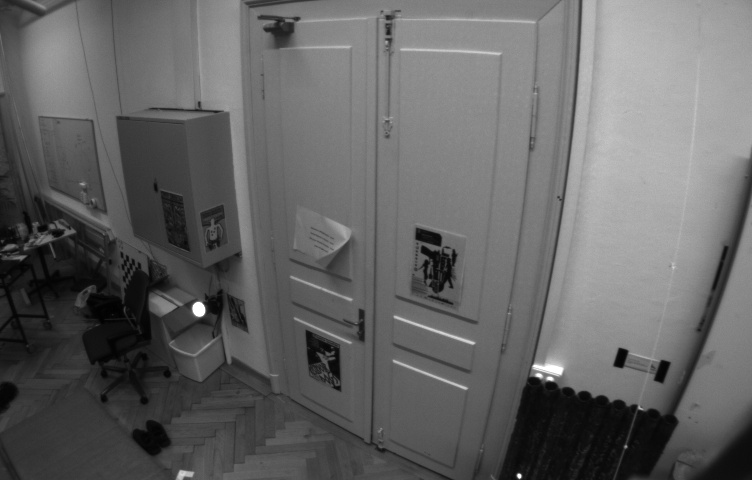
\includegraphics[width=0.75\textwidth]{images/frame0128}
  \caption{Frame from the \ac{UAV} data set}
  \label{fig:dataset_uav}
\end{figure}

\section{\acf{ROS} setup}
As already mentioned, the data set for the two clients were created by splitting a bigger data set recorded with only one client. Because the splitted data sets don't have the same timing, a retiming \ac{ROS} node, explained in the next subsection, was written to work around this issue.\\
To get the ground truth in a usable format, a record \ac{ROS} node, explained in \autoref{subsec:record_node}, was written which receives the ground truth position from the retimin \ac{ROS} node and writes it into a text file.\\

The whole \ac{ROS} setup is illustrated in \autoref{fig:ros_setup}.

\tikzstyle{block} = [draw, fill=white, rectangle, minimum height=3em, minimum width=6em]
\tikzstyle{point} = [coordinate]
\begin{figure}[H]
  \centering
  \begin{tikzpicture}[auto, node distance=2cm,>=latex']
		\node [block] (client_1) {rosbag for client 1};
		\node [point] (p1) [right= 1.0cm of client_1]{};
		\node [point] (p2) [below= 0.55cm of p1]{};
		
		\node [block] (client_2) [below = 1.5cm of client_1.west, anchor=west] {rosbag for client 2};	
		\node [point] (p3) [right = 1.0cm of client_2]{};
		\node [point] (p4) [above = 0.5cm of p3]{};
		
		\node [block] (retiming) [below right =-0.3cm and 2cm of client_1] {retiming node};
    \node [point] (p5) [right = 1cm of retiming, yshift=0.2cm]{};
    \node [point] (p7) [above = 0.9cm of p5]{};
    \node [point] (p6) [right = 1cm of retiming, yshift=-0.2cm]{};
    \node [point] (p8) [below = 0.9cm of p6]{};

    \node [block] (slam) [above right = 0.001cm and 2cm of retiming] {SLAM System};
    \node [block] (recording) [below right = 0.001cm and 2cm of retiming] {recording node};
		
		%\draw [-] (publish_image) -- node[name=u] {/cam0/image\_raw, /camera\_imu/vrpn\_client/estimated\_transform} (p1);
		%\draw [-] (publish_image) -- node[name=u] {grayscale images, ground truth positions} (p1);
		\draw [-] (client_1) -- node[name=u] {} (p1);
		\draw [-] (p1) -- (p2);
		\draw [-] (p3) -- (p4);
		
		\draw [-] (client_2) -- (p3);
		
		\draw [->] (p2) -- (p2-|retiming.west);
		\draw [->] (p4) -- (p4-|retiming.west);

    \draw [-] ([yshift=0.2cm]retiming.east) -- (p5);
    \draw [-] ([yshift=-0.2cm]retiming.east) -- (p6);

    \draw [-] (p5) -- (p7);
    \draw [-] (p6) -- (p8);

    \draw [->] (p7) -- (p7-|slam.west);
    \draw [->] (p8) -- (p8-|recording.west);
	\end{tikzpicture}
  \caption{\ac{ROS} setup}
  \label{fig:ros_setup}
\end{figure}

\subsection{Re-timing node}
The re-timing \ac{ROS} node subscribes to the topics providing the ground truth position and the greyscale image and republishes the messages of these topics with the time stamp set to the current system time.

\subsection{Recording node}
\label{subsec:record_node}
The recording \ac{ROS} node subscribes to the topic, the re-timing \ac{ROS} node publishes, which contains the ground truth position. It saves the ground truth positions into a list and at the end writes all the positions together with their time stamps into a text file.

\section{Evaluation}
To evaluate the proposed new map merging approach and to measure the influence of the culling as well as the change of the optimization algorithm to the accuracy an evaluation procedure was developed in this semester project. The evaluation procedure performs the following steps:

\begin{enumerate}
  \item Loads ground truth and \ac{SLAM} positions
  \item Find corresponding (in time) ground truth and \ac{SLAM} positions
  \item Perform a 7DoF alignment between the ground truth and the \ac{SLAM} positions
  \item Calculate the \acf{RMSE} between the ground truth and the \ac{SLAM} positions
\end{enumerate}

In the following subsections each step will be described in more detail.

\subsection{Loading of the ground truth and \ac{SLAM} positions}
This step involves the loading of the positions from the text files, applying the time offset $t_{\text{off}}$ and applying the camera-to-marker transformation $T_{\text{camera\_marker}}$.\\

The offset $t_{\text{off}}$ has to be applied as there is a time offset, emerging from the fact that the \ac{ROS} messages with the greyscale image and the \ac{ROS} messages with the ground truth position do not have the same time of travel, which has to be compensated.\\
For the \ac{UAV} data set the time offset varies a lot as both topic are received over a unreliable wireless LAN connection. To counteract this situation different time offset are tried by brute-forcing and the time offset which results in the smallest \ac{RMSE} is taken.\\ 

As the camera and the marker of the motion tracking system do not have the same position, the transformation $T_{\text{camera\_marker}}$ has to be applied that the ground truth positions and the \ac{SLAM} positions are in the same coordinate system for the evaluation.

\subsection{Find corresponding ground truth and \ac{SLAM} positions}
In this step for every \ac{SLAM} position the first ground truth position with a time stamp higher than the one of the \ac{SLAM} position is searched in line \autoref{line:corr1}. After that the absolute time difference between the time stamp of the \ac{SLAM} position and the time stamp of the ground truth position right before the one which was found in the previous step is calculated in line \autoref{line:corr2}. If this absolute time difference is smaller than the specified accuracy, the ground truth and the \ac{SLAM} positions are saved in a new array (lines \autoref{line:corr2}-\autoref{line:corr3}). The full procedure is listed in \autoref{lst:correspond}.

\lstset{language=Python}
\begin{lstlisting}[frame=single, caption=Find corresponding positions in time, label=lst:correspond]
def time_matching(list_gt_x,list_slam_x,gt_coordinates,
                  slam_coordinates,accuracy):

  # Matching of the datasets according to their time stamps
  gt = np.zeros((len(list_gt_x), 4))
  slam = np.zeros((len(list_slam_x), 4))

  pos = 0
  offset = 1
  break_flag = False
  for i in range(len(list_gt_x)):
    for j in range(offset, len(list_slam_x)):
      # value where slam time > gt time
      if gt_coordinates[i,0] < slam_coordinates[j,0]:|\label{line:corr1}|
        # check the one before
        if abs(gt_coordinates[i,0]-slam_coordinates[j-1,0])|\label{line:corr2}||\Suppressnumber|
                                                < accuracy:|\Reactivatenumber{17}|
          gt[pos] = gt_coordinates[i]
          slam[pos] = slam_coordinates[j - 1]|\label{line:corr3}|
          pos = pos + 1
          if pos >= len(slam_coordinates):
            break_flag = True
            break
          offset = j
          continue
    if break_flag==True:
      break

  # Remove empty rows
  slam = slam[~(slam == 0).all(1)]
  gt = gt[~(gt == 0).all(1)]

  return slam, gt
\end{lstlisting}

\subsection{Perform a 7DoF alignment}
A 7DoF alignment is necessary as monocular \ac{SLAM} systems, as the one this semester project is based on, doesn't provide a scale and position and rotation of the \ac{SLAM} coordinate system and the one of the ground truth doesn't have to be the same one.\\

To perform the 7DoF alignment an implementation of the algorithm proposed in \cite{Umeyama1991} was used. This algorithm determines the transformation and the scaling which results in the least \ac{RMSE}. With this transformation and scaling the \ac{SLAM} positions are transformed and scaled accordingly.

\subsection{Calculate the \acf{RMSE}}
The \acf{RMSE} between the ground truth and the \ac{SLAM} positions is calculated according to
\begin{equation}
  \textit{rmse} = \sqrt{\frac{1}{N - 1} \sum_i^N \big( (x_{\text{SLAM},i} - x_{\text{gt},i})^2 + (y_{\text{SLAM},i} - y_{\text{gt},i})^2 + (z_{\text{SLAM},i} - z_{\text{gt},i})^2\big)}
\end{equation}
where $N$ is the total number of positions, $x_{\text{SLAM},i}$, $y_{\text{SLAM},i}$ and $z_{\text{SLAM},i}$ are the positions of the \ac{SLAM} system and $x_{\text{gt},i}$, $y_{\text{gt},i}$ and $z_{\text{gt},i}$ are the ground truth positions provided by a motion tracking system.
